\documentclass[tikz,border=10pt]{standalone}

\begin{document}
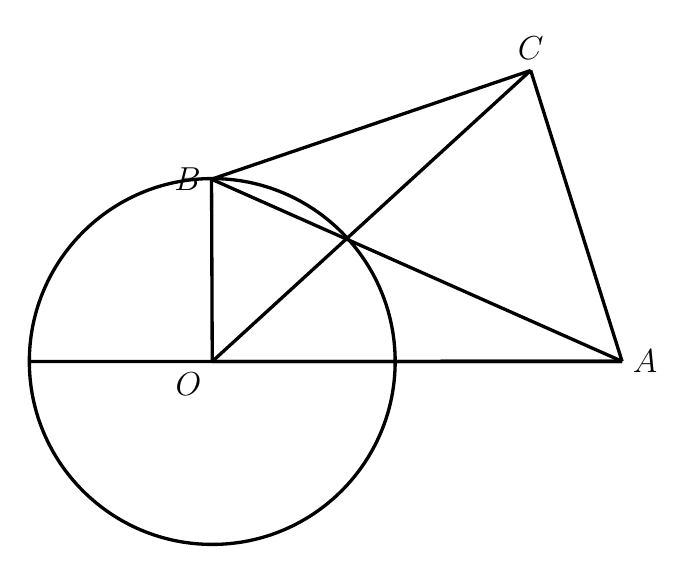
\begin{tikzpicture}[line width=1.2pt, line join=round]
\coordinate (A) at (3.460,-0.954);
\coordinate (B) at (-1.754,1.359);
\coordinate (C) at (2.299,2.740);
\coordinate (O) at (-1.745,-0.956);







  
  \draw (O) circle[radius=2.323];

  
  \draw (-4.063,-0.956) -- (O) -- (A);

  
  \draw (O) -- (A);

  
  \draw (O) -- (B);

  
  \draw (B) -- (A);
  \draw (C) -- (A);
  \draw (C) -- (O);
  \draw (C) -- (B);

  
  \node[right] at (A) {\fontsize{12.5}{15}\selectfont$A$};
  \node[left] at (B) {\fontsize{12.5}{15}\selectfont$B$};
  \node[above] at (C) {\fontsize{12.5}{15}\selectfont$C$};
  \node[below left] at (O) {\fontsize{12.5}{15}\selectfont$O$};
\end{tikzpicture}
\end{document}